\chapter{Zientzia konputazioa.}

\epigraph{Processor speed doubles every 18 months.}{\textit {Moore's Law (1965)}}
\epigraph{Number of cores per chip can double every two years.}{\textit Moore's Law Reinterpreter (2006)}

\section{Sarrera.}

Gaur-egungo konputagailuak (super-konputagailu, eramangarri,...) orokorrean paraleloak dira. 1986-2002 urteen artean, txip barruan transistore dentsitatea handitzen zen heinean, prozesadore bakarreko konputagailuen eraginkortasuna hobetuz joan zen. Baina teknologi-garapena muga fisikoetara iritsita, bide honetatik konputagailuen abiadura hobetzea ezinezkoa bilakatu zen (Irudia \ref{fig:51}). Horrela, 2005.urtetik aurrera fabrikatzaileek konputagailuen gaitasuna hobetzeko, txipan prozesadore bat baino gehiago erabiltzea erabaki zuten.      

\begin{figure}[h]
\centerline{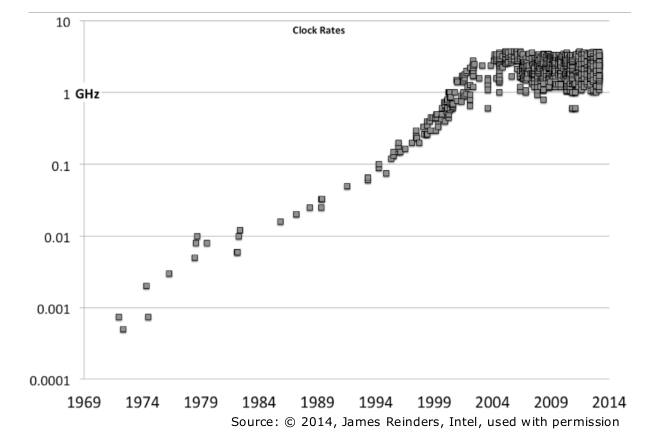
\includegraphics[width=10cm, height=6cm] {ProcessorClock}}
\caption[Processor clock rate.]{\small Processor clock rate growth halted around 2005.}
\label{fig:51}
\end{figure} 

%\begin{figure}[h]
%\centerline{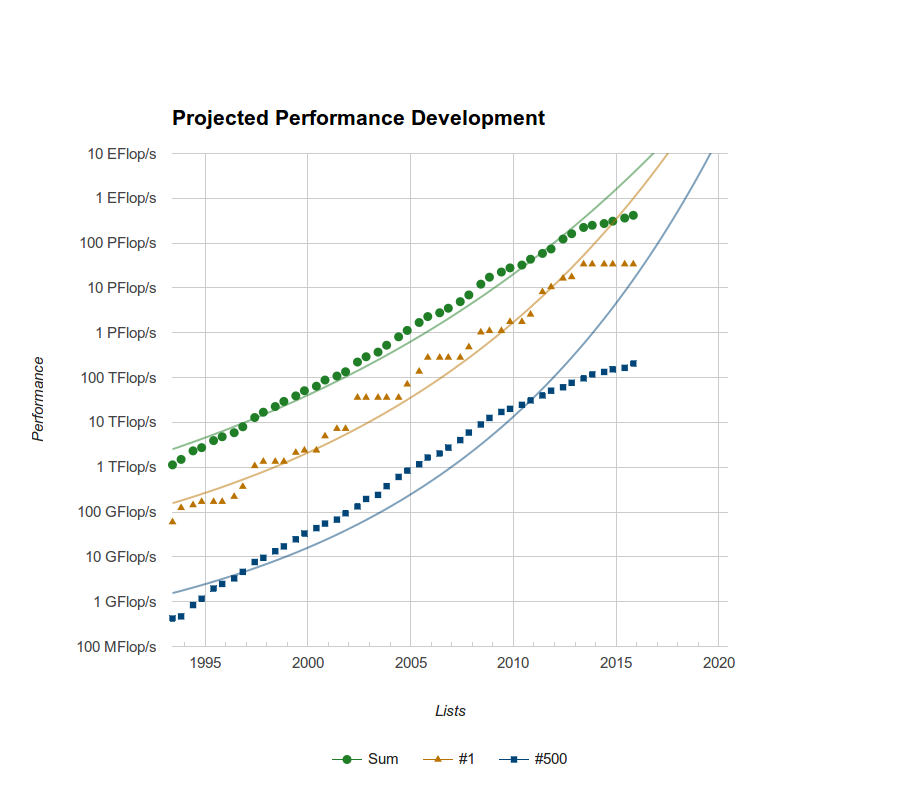
\includegraphics[width=12cm, height=8cm] {PerformanceDevelopment}}
%\caption[Konputagailuen eraginkortasuna.]{www.top500.org, Top: total computing power of top 500 computers. Middle: 1 %computer. Bottom: 500 computer.}
%\label{fig:61}
%\end{figure} 

Konputagailuen eredu aldaketa honen ondorioz, algoritmo azkarrak garatzeko kodearen paralelizazio gaitasunari heldu behar zaio. Programazio paralelo teknikak inplementatzeko, beharrezko da prozesadore berrien hardware arkitekturak nahiz software ingurune berriak ulertzea. Gaia nahiko konplexua izanik, ikuspegi orokorra eman ondoren, gure inplementazioan erabilitako hardware arkitektura eta software teknika zehatzak azalduko ditugu: memoria-konpartitutako sistemak eta OpenMP programazio eredua.

Bi dira, algoritmo azkarrak diseinatzeko erronkak: 
\begin{enumerate}
\item Paralizatzeko pisuko lana identifikatzea.
\item Memoria eta prozesadorearen arteko datu mugimendua gutxitzea. 
\end{enumerate}

Bestalde, inplementazio berrien garapenean optimizatutako liburutegiak erabiltzea komeni da. Horien artean, LAPACK eta BLAS algebra linealeko liburutegiak erabilgarriak izan zaizkigu. Liburutegi hauen gaineko azalpenak emango ditugu.

\section{Eraginkortasuna.}

\subsection*{\textbf{Zein azkarrak dira konputagailuak?}}

Gaur egungo prozesadoreen maiztasun-abiadura hertzetan neurtzen da, hau da,  \emph{makina ziklo segundoko} kopuruaren arabera. Une honetako prozesadoreak gigahertz mailakoak dira.
\begin{description}
\item {Kilo} = mila ($10^3$).
\item {Mega} = milioi ($10^6$).
\item {Giga} = bilioi ($10^9$).
\item {Tera} = trilioi ($10^{12}$).
\item {Peta} = $10^{15}$.
\item {Exa} = $10^{18}$. 
\end{description}

Koma-higikorreko oinarrizko eragiketa bat egiteko ($\oplus,\ominus,\otimes,\oslash$) ziklo gutxi batzuk behar dira. Honek esan nahi du, $1$ GHz-ko prozesadore batek,
$>100.000.000$ koma-higikorreko eragiketa segundoko egiten dituela ($>100$ megaflops).

\paragraph*{\textbf{Adibidea}.} 
Demagun $A,B$ eta $C \ (n \times n)$ dimentsioko matrizeak ditugula eta $C=AB$ matrize arteko biderketa egiteko behar dugun denbora jakin nahi dugula.
\begin{equation*}
c_{ij}=\sum\limits_{i,j=1}^{n} a_{ij}*b_{ji}.
\end{equation*}

\begin{itemize}
\item $c_{ij}$ gai bakoitza kalkulatzeko $n$ biderketa eta ($n-1$) batura egin behar ditugu.
\item $C$ matrizeak $n^2$ osagaia ditu $\Rightarrow$ $O(n^3)$ koma-higikorrezko ariketak exekutatu behar dira.
\end{itemize}

Adibidez, $n=100$ bada $\ \Rightarrow \ n^3=10^{6}$ eragiketa egin behar ditugu. $1$GHz prozesadorean exekutatzeko, $>10^(-2)$ segundo beharko genituzke. 

\paragraph*{} Zientzia konputazioaren eraginkortasuna neurtzeko, koma-higikorreko eragiketa kopurua (\emph{flops}) erabili ohi zen. Problema handia denean, datuen mugimendua koma-higikorreko eragiketak baino garestiagoa da, eta beraz eraginkortasuna eragiketa kopuruaren arabera neurtzea okerra izan daiteke. Kodearen exekuzioa azkartzeko derrigorrezkoa da konputagailuan datuen mugimendua minimizatzea.

\paragraph*{\textbf{Adibidea},} $n=400$ tamainako matrizeak hartzen baditugu, $15,6$ \emph{MB} memoria behar dugu (suposatuz konputagailuaren CACHE memoria baino handiagoa) eta datuen mugimenduaren eragina nabarituko da exekuzio denboran.

\subsubsection*{Timing code.}

Unix \emph{time} agindua erabili daiteke, konputazioen denborak ezagutzeko:

\begin{lstlisting} 
S time ./a.out
<kodearen irteera>

real 0m38.856s
user 0m38.789s
sys  0m0.004s
\end{lstlisting}

Agindu honekin, \emph{./a.out} C programa exekutatuko da eta ondoren, programa exekutatzeko behar izan duen denboraren informazioa pantailaratuko du: \emph{real} hasi eta bukatu arteko denbora (\emph{wall-time}); \emph{user} prozesadoreak gure programa exekutatzen erabili duen denbora (\emph{CPU-time}); \emph{sys} programa exekutatu ahal izateko, sistema eragile lanetan emandako denbora.   

\paragraph*{} C lengoaian badaude, denbora neurtzeko funtzioak. Jarraian, exekuzio denbora (\emph{Wall-time}) eta cpu denborak \emph{CPU-time} nola kalkulatu azaldu dugu.

\begin{lstlisting}[language=C]

#include <time.h>

    time_t  wtime0,wtime1;
    clock_t clock0, clock1; 

    wtime0= time(NULL);
    clock0= clock();

    <neurtu nahi den kodea>

    wtime1= time(NULL);
    clock1=clock();
    
    Wall_time=(wtime1 - wtime0);
    CPU_Time=(clock1 - clock0)/CLOCKS_PER_SEC);

\end{lstlisting}

\emph{Wall-time} deiturikoa izango da algoritmo baten denborak neurtzeko gure irizpidea. Programazio paraleloan, algoritmoen exekuzio denborak egokien neurtzen duen aldagaia da. Dena den, une berean programa bakarra exekutatzea behartuta gaude.       
 

\section{Hardwarea.}

\subsection{Memori hierarkia.}

Lehenik, konputagailuan dauden memoria mota ezberdinen hierarkia azalduko dugu. 
\begin{figure}[h]
\centerline{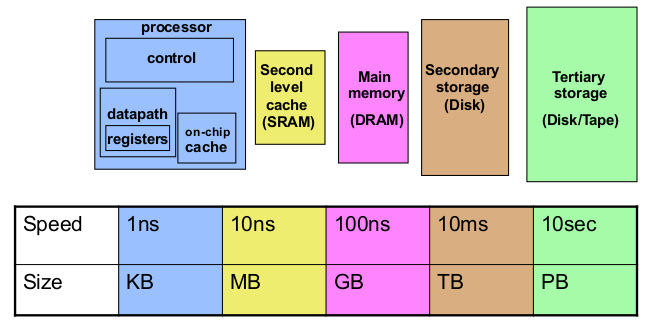
\includegraphics[width=10cm, height=4cm] {MemoryHierarchy}}
\caption{Memoria hierarkia.}
\label{fig:three}
\end{figure} 

\paragraph*{} CPU-k koma-higikorrezko eragiketak egiten ditu: erregistroetatik datuak irakurri, eragiketak egin eta emaitza erregistroetan idazten ditu. Memoria nagusia eta erregistroen artean, 2 edo 3 mailako Cache memoria dugu: lehen Cache memoria (L1) txikiena eta azkarrena da, eta beste mailak (L2,L3,...), handiagoak eta motelagoak. Memoria nagusian, exekutatzen diren programak eta datuak gordetzen dira ($1-4$ GB artekoa). Azkenik, disko gogorrean konputagailuko datu (argazki, bideo,...) eta erabilgarri ditugun programa guztiak gordetzen dira.  

Cache memoria lerroka egituratuta dago eta lerro bakoitza $64$ edo $128$ bytez ($8$ edo $16$ double zenbaki) osatuta dago. Programa batek datu bat behar duenean, memoria nagusitik lerro tamainako datu taldea irakurriko du eta Cachean idatziko ditu. Komunikazio hau minimizatzeko memorian datuak gordetzeko ordenak badu garrantzia. Beraz, datu-egiturak diseinatzen direnean, kontutan hartu behar da une berean beharko diren datuak memorian gertu gordetzea   

\paragraph*{\textbf{Adibidea}.}Badakigunez, C-lengoaian matrizeak lerroka gordetzen dira. Beheko adibidean,  matrizearen lehen osagaia $a(1,1)$ behar dugunean, memoria nagusitik Cachera osagai honetaz gain jarraiko 16 osagaiak ekarriko dira ($a(1,1),a(1,2),\dots,a(1,16)$). Honela, hurrengo $15$ batura egiteko behar ditugun datuak Cachean eskuara izango ditugu memoria irakurketa berririk egin gabe. 

\begin{algorithm}[h]
 \BlankLine
  $int \ n$\;
  $double \ a[n][m]$\;
  \BlankLine
  $sum=0$\;
  \For{$i\leftarrow 1$ \KwTo $n$}
  {
   \BlankLine
    \For{$j\leftarrow 1$ \KwTo $m$}
   {
    \BlankLine 
    $sum+=a(i,j)$\;
   }
 }
 \caption{Memoria atzipena.}
\end{algorithm} 

\begin{equation*}
a=\left(\begin{array}{ccccc}
  1    & 2    & 3    & \dots & 1000 \\
  1001 & 1002 & 1003 &\dots & 2000 \\
  2001 & 2002 & 2003 &\dots & 2000 \\
  \dots & \dots & \dots & \dots & \dots \\
  9001 & 9002 & 9003 &\dots & 10000 \\
  \end{array}\right).  
\end{equation*}

\paragraph*{}CPUk datu bat behar duenean, memoria hierarkian zehar bilatuko du: lehenik $L1$ cachean, ondoren $L2$ cachean,...eta hauetan ez badago, memoria nagusira joko du. Memoria nagusi eta cache memoria arteko irakurketa eta idazketa guzti hauetan,  informazio konsistentzia mantentzeko hainbat arau aurrera ematen dira.  

\subsection{Hardware motak.}

MIMD (Multiple instruction, multiple data) sistemak, guztiz independenteak diren prozesadore multzoak osatzen dituzte. Bi dira MIMD sistema nagusiak: memoria konpartitutako eta memoria banatutako sistemak. Memoria konpartitutako sistemetan, prozesadore guztiek memoria osoa konpartitzen dute eta inplizituki konpartitutako datuen atzipenaren bidez komunikatzen dira. Memoria banatutakotako sistemetan aldiz, prozesadore bakoitzak bere memoria pribatua du eta esplizituki bidalitako mezuen bidez komunikatzen dira.

Hirugarren hardware arkitektura ere aipatuko dugu, general purpose GPU computing (Graphical Processor Unit).
Jokoen eta animazio industrian, grafiko oso azkarrak beharrak bultzatuta  sortutako teknologia da. Oinarrian, imajinak pantailaratzeko prozesagailu asko paraleloan lan egiten dute. Azken hamarkadan, GPU unitate hauek zientzia konputaziora zabaldu dira.  

\begin{figure}[h]
\centerline{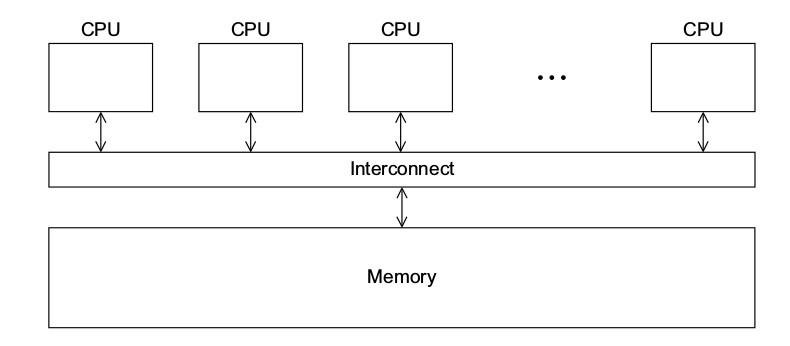
\includegraphics[width=12cm, height=4cm] {SharedMemorySystem}}
\caption{Memoria konpartitutako sistemak.}
\label{fig:61}
\end{figure}  

\begin{figure}[h]
\centerline{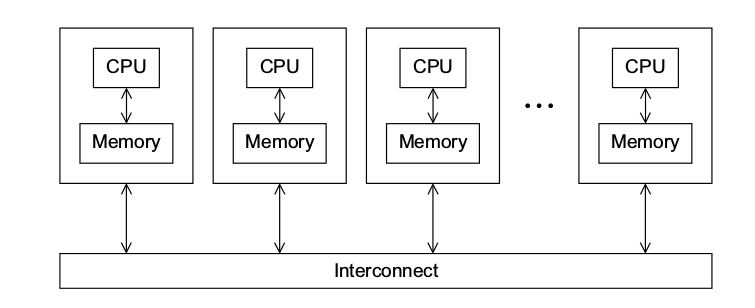
\includegraphics[width=12cm, height=4cm] {DistribuitedMemorySystem}}
\caption{Memoria banatutako sistemak.}
\label{fig:61}
\end{figure}  

\paragraph*{\textbf{Memoria konpartitutako sistemak}.}

Multicore bat edo gehiagoz osatutako sistema dugu. Multicore prozesadore bakoitzak txipean CPU bat baino gehiago ditu. Normalean CPU bakoitzak $L1$ bere cache memoria du. Aipatzeko da, era honetako sistemetan prozesadore kopurua ezin dela nahi adina handitu eta mugatua dela (normalean $\leq 32$ ).

 \begin{figure}[h]
 \centerline{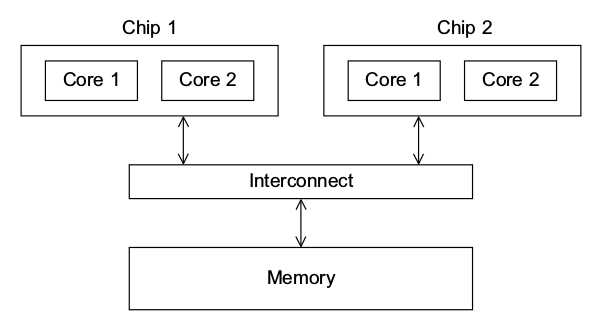
\includegraphics[width=12cm, height=4cm] {SharedMemorySystemUMA}}
 \caption{Memoria konpartitutako sistemak (UMA).}
 \label{fig:61}
 \end{figure}  

\section{Softwarea.}


\subsection{Software liburutegiak.}

Matematika bi software errekurtso nagusienak aipatuko ditugu; BLAS (Basic Linear Algebra Subroutines) eta LAPACK (Linear Algebra Package). Kalitate handiko software orokorrak dira eta hauek erabiltzea abantaila asko ditu: 
\begin{enumerate}
\item Garapen berriak egiteko denbora aurrezten da. 
\item Problema askotan ondo probatutako softwareak dira.
\item Konplexutasun handikoak dira, modu seguruan eta azkarrean exekutatzeko diseinatu direlako. 
\end{enumerate}

Konputagailu hardware bakoitzerako optimizatutako bertsioak daude. Inplementazioa Fortranen egina dago eta datu-motei dagokionez:
\begin{enumerate}
\item S: float ($32$ bit).
\item D: double ($64$ bit).
\item C: complex.
\item Z: complex double.
\end{enumerate}   

\subsubsection*{\textbf{BLAS}.}

BLAS liburutegian, bektore eta matrizeen arteko funtzio estandarrak inplementatuta daude. Hiru mailetan banatuta dago: 

\begin{enumerate}
\item BLAS-1: bektore-bektore eragiketak.

 Adibidez: $y=\alpha*x+y$ , $2n$ flop eta $3n$ irakurketa/idazketa.
 
 Konputazio intentsitatea: $\frac{2n}{3n}=\frac{2}{3}$. 

\item BLAS-2: matrize-bektore eragiketak.

 Adibidez: $y=\alpha*A*x+\beta*x$, $O(n^2)$ flop eta $O(n^2)$ irakurketa/idazketa.
 
 Konputazio intentsitatea: $\approx \frac{2n^2}{n^2}=2$. 
 
\item BLAS-3: matrize-matrize eragiketak.

 Adibidez: $C=\alpha*A*B+\beta*C$, $O(n^3)$ flop eta $O(n^2)$ irakurketa/idazketa.
 
 Konputazio intentsitatea: $\approx \frac{2n^3}{4n^2}=\frac{n}{2}$. 

\end{enumerate}

Azpimarratu, BLAS-1 eta BLAS-2 funtzioen konputazio intentsitatea txikia dela eta beraz, datuen komunikazioa nagusia dela. BLAS-3 aldiz, konputazio intentsitatea handiagoa da eta ezaugarri honi esker, konputagailuaren konputazio gaitasuna ondo aprobetxatu ahal izango da.

\begin{figure}[h]
\centerline{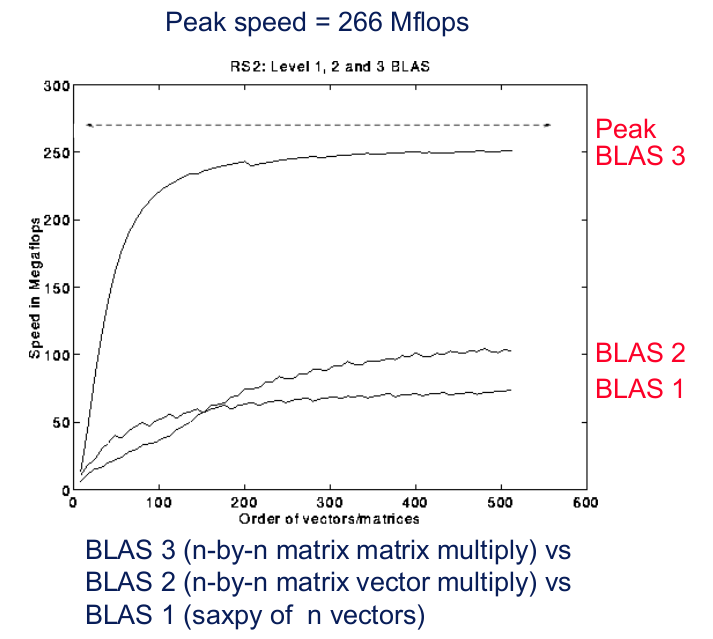
\includegraphics[width=12cm, height=8cm] {BLASSpeed}}
\caption{BLAS speeds.}
\label{fig:61}
\end{figure}    

Fabrikatzaile bakoitzak optimizatutako BLAS liburutegiak (AMD ACML,Intel MKL) dituzte eta beraz, multi-threaded dira.
Beste aukera bat, optimizatutako BLAS instalazioa ATLAS (Automatically Tuned Linear Algebra Software) bidez egitea.    

\subsubsection*{\textbf{LAPACK}}.

Zenbakizko aljebra linealaren liburutegia da.

\begin{enumerate}
\item Sistema linealak: $AX=b$.
\item Least Square: choose $x$ to minimize $\|Ax-b\|$.
\item Eigenvalues.
\item Balio singularren deskonposaketa (SVD).
\end{enumerate}

Posible den guztietan, BLAS-3 funtzioetan oinarritzen da.

\subsection{Programazio paraleloa.}

C-lengoaia programazio paraleloan erabiltzeko, lengoaiaren bi extensio dira nagusienak: bata memori-banatutako sistemetarako diseinatuta  MPI (Message-Passing Inteface) eta bestea, memoria-konpartitutako sistemetarako diseinutakoa OpenMP (Open Specifications for MultiProcessing). MPI datu moten definizio, funtzio eta makroen liburutegia da. OpenMP liburutegia bat  eta C konpiladorearen aldaketa batzuk. OpenMP erabili dugu gure inplementaziorako eta jarraian honi buruzko idei nagusienak emango ditugu.

\paragraph*{\textbf{OpenMP}.}

Memoria konpartitutako programazio paraleloaren estandarra dugu. 
Programazioan paralelizazio kontrola, "fork-join" modeloa jarraituz egiten da.

\begin{enumerate}
\item OpenMP programen hasieran prozesu bakarra dago, hari (thread) nagusia. 
\item FORK: hari nagusiak hari talde paraleloa sortzen du.
\item JOIN: hariak kode paraleloa bukatzen dutenean, behin sinkronizatuta amaitzen dute eta hari nagusiak bakarrik jarraitzen du.
\end{enumerate}

% \begin{figure}[h]
% \centerline{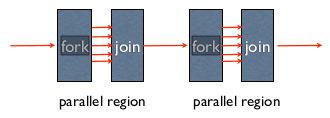
\includegraphics[width=10cm, height=3cm] {ForkJoin}}
% \caption{Fork-Join.}
% \label{fig:61}
% \end{figure}  
 
 \begin{figure}[h]
 \centering
 \subfloat[Fork-Join.]{
 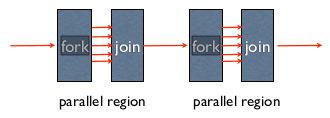
\includegraphics[width=.500\textwidth]{ForkJoin}
 }
 \subfloat[Fork-Join.]{
 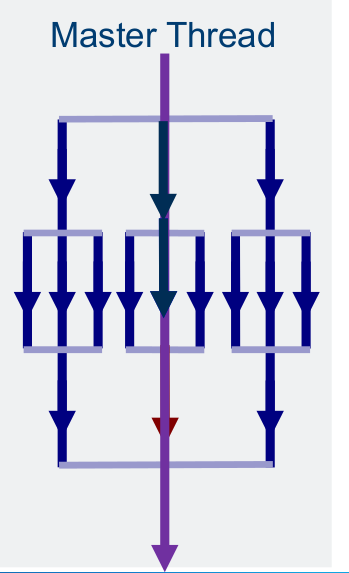
\includegraphics[width=.200\textwidth]{OpenMP1}
 }
  \caption[OpenMp programazio modeloa.]{\small OpenMp programazio modeloa.}
 \label{fig:forkjoin}
 \end{figure}

Aldagai batean (threadcount) paralelizazioan zenbat hari erabili adierazten da eta ohikoa izaten da hari bat prozesadore bakoitzeko sortzea.  Konpilazio direktiben bidez,  paralelizazioa nola exekutatu behar den zehazten zaio.

\paragraph*{\textbf{Adibidea}}.

\begin{lstlisting}[language=C]
#    pragma omp parallel for num_threads(thread_count) 
     for (i = 0; i<n; i++)
     {
       ! Aginduak 
     }
\end{lstlisting}

OpenMP Version 4.5.	

gcc -v (gcc version 4.8.4 (Ubuntu 4.8.4-2ubuntu1~14.04.3))

A number of compilers from various vendors or open source communities implement the OpenMP API:

\begin{enumerate}
\item From GCC 4.7.0, OpenMP 3.1 is fully supported. 

\item From GCC 6.1, OpenMP 4.5 is fully supported in C and C++.

\end{enumerate}   


\subsection{Konpiladorea.}

\subsubsection*{Sarrera.}

Erabiliko dugun konpiladorea,

\begin{enumerate}

\item \emph{gcc} - \emph{GNU} open source compiler.

\begin{lstlisting}
$ gcc -v
$ gcc version 4.8.4 (Ubuntu 4.8.4-2ubuntu1~14.04.3) 
\end{lstlisting}

\item Several comercial compilers also are avalaible.

\end{enumerate}


C11 (formerly C1X) is an informal name for ISO/IEC 9899:2011,[1] the current standard for the C programming language.It replaces the previous C standard, informally known as C99. This new version mainly standardizes features that have already been supported by common contemporary compilers, and includes a detailed memory model to better support multiple threads of execution.

gcc requires you specify -std=c99 or -std=c11


\paragraph*{Optimizations} (-Olevel).
        
Optimizes the code for execution speed according to the level specified by level , which can be 1, 2, or 3. If no level is specified, as in –O , then 1 is the default. Larger numbers  indicate higher levels of optimization.

-O2 (default) Optimize for code speed. This is the generally recommended optimization level. -O3 Enable -O2 optimizations and in addition, enable more aggressive optimizations such as loop and memory access transformation, and prefetching. 

Every compiler offers a collection of standard optimization options (-O0,-O1,. . . ).  However, all compilers refrain from most optimizations at level -O0, which is hence the correct choice for analyzing the code with a debugger. At higher levels, optimizing compilers mix up source lines, detect and eliminate “redundant” variables, rearrange arithmetic expressions, etc.,      

\subsubsection*{Konpilazioa.}

\paragraph*{Oinarrizko erabilpena.}

\begin{enumerate}
\item Compiles and links and creates an executable adibidea.exe.
\begin{lstlisting}[language=C]
$ gcc adibidea.c -o adibidea.exe
\end{lstlisting}

\begin{lstlisting}[language=C]
$ ./adibidea.exe
\end{lstlisting}

\item Compile and link steps.

\begin{lstlisting}[language=C]
$ gcc adibidea.c  # creates adibidea.o
$ gcc adibidea.o -o adibidea.exe
\end{lstlisting}

\end{enumerate}

\begin{lstlisting}[language=C]
gcc -O2 -Wall -std=c99 -fno-common adibidea.c
\end{lstlisting}

\subsubsection*{Makefile.}

A common way of automating software builds and other complex tasks with dependencies.

A Makefile is itself a program in a special language.

\paragraph*{Adibidea.}
Demangun programa bat hiru fitxategieten banatuta dugula,

\begin{lstlisting}[language=C]
/*file: main.c*/
void main()
{
    printf("Main program");
    sub1();
    sub2();
}
\end{lstlisting}

\begin{lstlisting}[language=C]
/*file: sub1.c*/
void sub1()
{
    printf("sub1");
}
\end{lstlisting}

\begin{lstlisting}[language=C]
/*file: sub2.c*/
void sub2()
{
    printf("sub2");
}
\end{lstlisting}

Programa exekutagarria lortzeko makefile fitxategia,

\begin{lstlisting} [language=C]
main.exe: main.o sub1.o sub2.o
	      gcc main.o sub1.o sub2.o -o main.exe
main.o: main.c
        gcc -c main.c
sub1.o: sub1.c
        gcc -c sub1.c        
sub2.o: sub2.c
        gcc -c sub2.c        
\end{lstlisting}

\begin{lstlisting}
$ make main.exe
gcc -c main.c
gcc -c sub1.c
gcc -c sub2.c
gcc main.o sub1.o sub2.o -o main.exe
\end{lstlisting}

Typical element in the simple Makefile:

\begin{lstlisting}
target: dependencies
>TAB>  command(s) to make the target
\end{lstlisting}

Typing "make target" means:
\begin{itemize}
\item Make sure all dependencies are update (those that are also targets).
\item If target older than any dependency, recreate it using specified commands.
\item The rules are applied recursively.
\end{itemize}

\paragraph*{\textbf{MakefileV2}}

\begin{lstlisting} [language=C]

CC = /usr/bin/gcc
FLAGS=-O2 -Wall -std=c99 -fno-common 
OBJECTS=  main.o sub1.o sub2.o
.PHONY: clean help

main.exe: $(OBJECTS)
	      ${CC} $(OBJECTS) -o main.exe
	      
%.o: %.c
     ${CC} ${FLAGS} -c $<	      
	      
clean:
     rm -f $(OBJECTS) main.exe

help:
    @echo "Valid targets;"
    @echo " main.exe"
    @echo " main.o"
    @echo " sub1.o"
    @echo " sub2.o"
    @echo " clean"
             
\end{lstlisting}


\section{Kode Optimizazioak.}

Applications have two general challenges:
\begin{enumerate}
\item Numerical Method.

Performance required computation the shortest account of time.

\item. Computer Program.

Express the algorithm as fast computer problem, you have realized computer hardware eficiently.

\end{enumerate}

Optimization areas are:
\begin{enumerate}
\item Vectorization.
\item Paralelization.
\item Memory trafic control.
\end{enumerate}

Optimization areas:
\begin{enumerate}
\item scalar optimization (compiler friendly practices).

\item vectorization (must use 16 or 8 wide vectors).

\item multi-threading (must  scale to $100+$ threads).

\item memory access (streaming acces).

\item communication (offload, MPI traffic control).

\end{enumerate}


\subsection*{Scalar Tuning and General Optimization.}

Optimization of scalar arithmetics.

One of the most important scalar optimizazion techincs is  \textbf{strength reduction} : replace expensive operation for less expensive operations.

\begin{figure}[h]
 \centerline{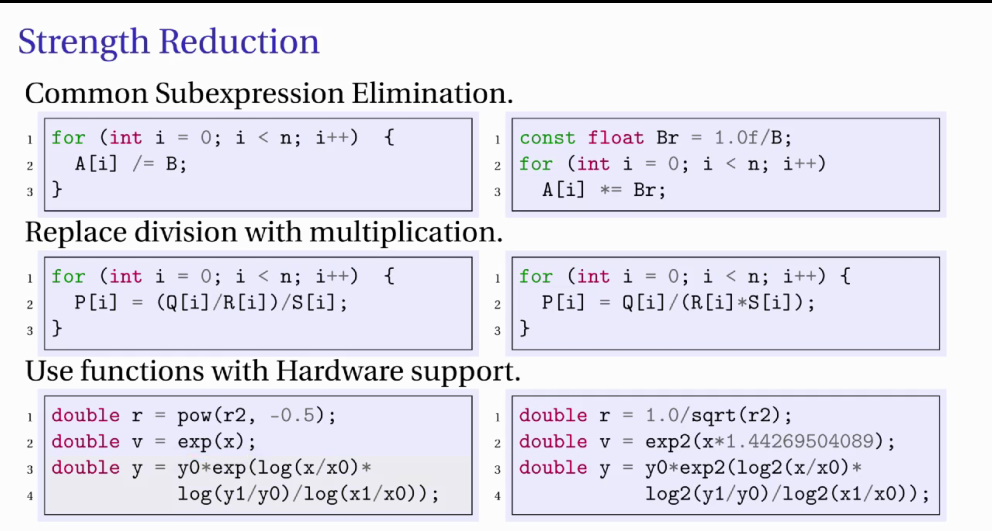
\includegraphics[width=12cm, height=4cm] {Optimization_Strength_Reduction}}
 \caption{Optimization.}
 \label{fig:61}
\end{figure}  

\paragraph*{} Precision control.

\begin{enumerate}
\item Precision Control for transcendental functions.

\item Floating-point semantics.

\item Consistency of precision: constants and constants.

Using incorrect function names in the single precsion is a common mistake

\end{enumerate}

\subsection*{Optimization of vectorization.}

\begin{enumerate}

\item Preferably unid-stride access to data.
Very important step in the optimization.

Artikulua "Auto-Vectorization with the Intel Compilers".

Most CPU architectures today include Single Instruction Multiple Data (SIMD) parallelism in the form
of a vector instruction set. Serial codes (i.e., running with a single thread), as well as instruction-parallel cal-
culations (running with several threads) can take advantage of SIMD instructions and significantly increase
the performance of some computations. Each CPU core performs SIMD operations on several numbers (in-
tegers, single or double precision floating-point numbers) simultaneously, when these variables are loaded
into the processor’s vector registers, and a vector instruction is applied to them. SIMD instructions include
common arithmetic operations (addition, subtraction, multiplication and division), as well as comparisons,
reduction and bit-masked operations (see, e.g., the list of SSE 2 intrinsics). Libraries such as the Intel Math
Library provide SIMD implementations of common transcendental functions, and other libraries provide
vectorized higher-level operations for linear algebra, signal analysis, statistics, etc.

\item Data Alignment and Padding.

An important consideration for efficient vectorization is data alignment.


\end{enumerate}

\subsection*{Multi-threading.}

Do you have enough parallelism in your code? 

Expanding iteration space, if it is no enough iterations in parallel loop.

Three layers of parallelism: MPI processes, OpenMP threads, vectorization.


\subsection*{Memory access.}

Memory access and Cache utilization.

loop tiling technics

\begin{figure}[h]
 \centerline{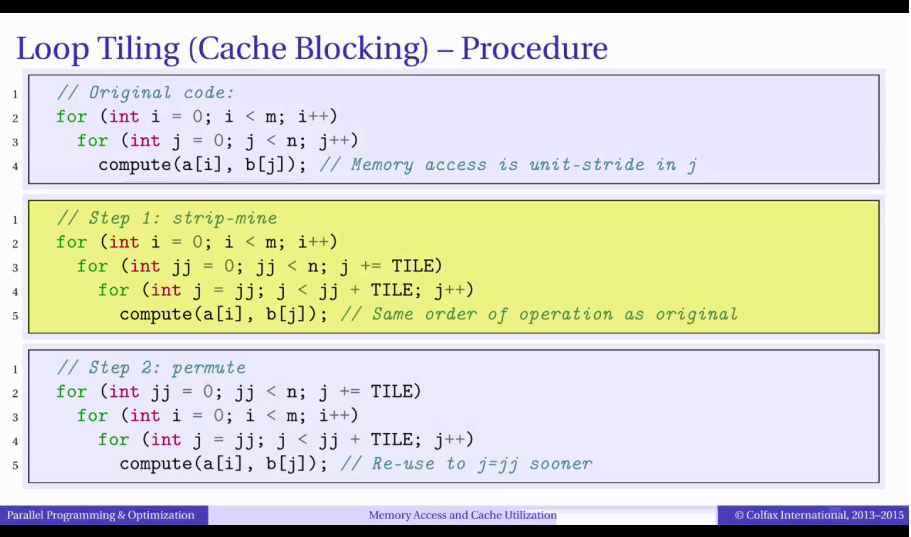
\includegraphics[width=12cm, height=4cm] {Optimization_LoopTiling}}
 \caption{Optimization.}
 \label{fig:61}
\end{figure}  

\section{Laburpena.}

Best practices for code vectorization and parallelization, and additional tips and tricks.

Algoritmo bat inplementatzen dugunean kontutan hartu beharrekoa:

\begin{enumerate}

\item Lerro edo zutabe araberako iterazioak exekuzio denboran eragin handia du.

\item Kodea garbia eta ulergarria mantendu behar da.

\item Badaude kodearen exekuzio denboraren analisia egiteko tresnak (adibidez gprof). Algoritmoaren funtzio bakoitzaren exekuzio denborari buruzko informazio erabilgarria lortuko dugu. Zenbait gauza modu sinplean azkartu daitezke baina zenbait beste gauza azkartzeko esfuertzu handia eskatu dezake.

\item Optimizatutako beste hainbat kode erabiltzea komenigarria da. LAPACK aljebra lineal paketea Fortran eta C-lengoaitetatik deitu daiteke. Eraberean, LAPACKek BLAS subrutinak erabiltzen ditu.  Subrutinak hauek matrizen arteko biderketak, "inner product", ... BLAS konputagailu arkitektura ezberdinetarako optimizatutako bertsioak daude.
 

\end{enumerate}

